
\subsection{Polynomial Encoding}
\label{sec:encoding}
At the heart of our protocol is an encoding of integer polynomials with bounded coefficients as integers with useful homomorphic properties. To extend the encoding to polynomials over an odd prime field $\mathbb{F}_p$, we first lift them to the ring of polynomials over the integers by selecting representatives from $\{-\frac{p-1}{2}, \ldots, \frac{p-1}{2}\}$ for each coefficient. The lifted polynomial has bounded integer coefficients and can hence be mapped into the integers.

We write $\ZZ(b):=\{x \in \ZZ \, | \, \vert x \vert  \leq b\}$ as the set of integers with absolute value less than or equal to $b$. In a slight abuse of notation we write $\ZZ(b)[X]\subset \mathbb{Z}[X]$ as the set of integer polynomials with bounded coefficients. 

\paragraph{Encoding}
For a ``large'' integer $q$, the map $\mathsf{Enc} : \mathbb{Z}((q-1)/2)[X] \rightarrow \mathbb{Z}, \, f(X) \mapsto f(q)$ is an injective map from the domain of polynomials with bounded coefficients to the integers. This means the map can be used as encoding of polynomials in the domain $\ZZ(b)[X]$ with $b<q/2$.
\paragraph{Decoding}
Decoding works as follows. Define the partial sum $S_k := \sum_{i=0}^k f_i q^i$ with $S_{-1} := 0$ and observe that when $(S_k \bmod q^{k+1}) > q^{k+1}/2$ then $S_k < 0$ whereas when $(S_k \bmod q^{k+1}) < q^{k+1}/2$ then $S_k \geq 0$. 
So when decoding $y \in \mathbb{Z}$, we can get $S_k$ for any $k$ by setting $S_k$ to $y \bmod q^{k+1}$ if $y \bmod q^{k+1}$ is less than $\frac{q^{k+1}}{2}$ or to $q^{k+1}- (y \bmod q^{k+1})$ otherwise.
Two consecutive partial sums yield a coefficient of $f(X)$: $f_k = \frac{S_{k} - S_{k-1}}{q^{k}} \in \ZZ(b)$. These operations give rise to the following algorithm.\\
\begin{minipage}{\textwidth}
\begin{mdframed}
\begin{flushleft}
	$\pro{Dec}(y \in \mathbb{Z}):$
	\begin{enumerate}[nolistsep]
	    \item \textbf{for each} $k$ \textbf{in} $[0, \, \lfloor \log_q(|y|)\rfloor]$ \textbf{do:}\\
		\item \pcind[1] $S_{k-1} \gets (y \bmod q^{k})$
		\item \pcind[1] \pcif{$S_{k-1} > q^{k}/2$} \textbf{then} $S_{k-1} \gets q^{k}-S_{k-1}$ \textbf{end if}
		\item \pcind[1] $S_k \gets (y \bmod q^{k+1})$
		\item \pcind[1] \pcif{$S_{k} > q^{k+1}/2$} \textbf{then} $S_{k} \gets q^{k+1}-S_{k}$ \textbf{end if}
		\item \pcind[1] $f_k \gets (S_{k} - S_{k-1}) / q^k$
		\item \pcreturn $f(X) = \sum_{i=0}^{\lfloor \log_q(|y|)\rfloor} f_i X^i$
	\end{enumerate} 
\end{flushleft}
\end{mdframed}
\end{minipage}

\begin{fact}
	The encoding scheme is uniquely decodable for polynomials in $\ZZ(b)[X]$ if $b<q/2$.
\end{fact}
The fact follows from $f(q)\in \ZZ$ being a unique integer representation of polynomials with coefficients bounded in absolute value by $b$ such that $b<q/2$. In particular for any partial sum $S_i$ we have $|S_i|<\frac{q^{i+1}}{2}$. From this it follows that $S_i-S_{k-i}=f_i \cdot q^i$.  

Note that the encoding has limited homomorphic properties: $\enc(g(X))+\enc(h(X))=\enc(g(X)+h(X))$ if $g(X)+h(X)\in \ZZ(b)$, \emph{i.e.}, if all its coefficients are less than $q/2$ in absolute value. This constraint is satisfied for example if the coefficients of $g$ and $h$ are less than $q/4$ in magnitude. Additionally, $\enc(g(X))\cdot \enc(h(X))=\enc(g(X)\cdot h(X))$ if $g(X)\cdot h(X)\in \ZZ(b)$.

\paragraph{Encoding of dyadic rational polynomials.}
In class groups there exists an algorithm to compute square roots of any element originally described by Gauß (modern description by Bosma and Stevenhagen~\cite{jtn/BosSte96}). As a result, in class groups an adversary can also commit to \defn{dyadic rationals} $\mathbb{D}:=\{\frac{x}{2^k} : \ x \in \ZZ \wedge k \in \NN\}\subset \QQ$, in addition to integers. When using class groups we therefore need to extend the encoding scheme accordingly. 

The encoding map is identical, except lifted to the dyadic rationals: $\mathsf{Enc} : \mathbb{D}[X] \rightarrow \mathbb{D}, \, g(X) \mapsto g(q)$. The main difference with respect to the integer encoding scheme will be that decoding works for dyadic rationals where \emph{both the numerator and the denominator are bounded}. Let $N \in \NN$ be a bound on the absolute value of the numerator and $2^D\in \NN$ be a bound on the value of the denominator, and let $\mathbb{D}(N, D) :=\{\frac{x}{2^a} \in \mathbb{D} : \ |x|\leq N \wedge 2^a \leq D\}$ denote the set of such bounded dyadic rationals. The encoding scheme is uniquely decodable if $N \cdot 2^a < q/2$.
 
Note that denominator of $g(q)$ is bounded by $2^{\lfloor\log_2(D)\rfloor}$, $D$ rounded down to the next power of $2$. To decode such a dyadic rational, compute the integer $y \gets g(q) \cdot 2^{\lfloor\log_2(D)\rfloor}\in \ZZ$  and use the decoding algorithm described above to decode a polynomial $f(X)$ in $\ZZ(q/2)[X]$. From $f(X)$ one derives the polynomial  $g(X) \gets \frac{f(X)}{2^{\lfloor\log_2(D)\rfloor}} \in \mathbb{D}(\lceil q/(2D)\rceil, 2^{\lfloor\log_2(D)\rfloor})[X]$ through division. If the integer polynomial encoding is uniquely decodable, then so is the scheme for dyadic rational polynomials. If $q$ is a power of $2$, then an adversary can encode Laurent polynomials, \emph{i.e.}, polynomials where some terms have negative powers. In order to disallow negative powers, $q$ must be odd.

\subsection{Information-Theoretical Polynomial Commitment Scheme}

Before we present our concrete polynomial commitment scheme based on groups of unknown order, we present an abstraction thereof that hides the concrete cryptographic steps. The purpose of this abstraction is two-fold: first, it provides an intuitive stepping stone from which presenting and studying the concrete cryptographic protocol is easier; and second, it opens the door to alternative cryptographic instantiations that provide the same interface but based on alternative hardness assumptions.

Let $[\![ \cdot ]\!] : \mathbb{Z}_p[X] \rightarrow \mathbb{S}$ be a homomorphic commitment function that sends polynomials over a prime field to elements of some set $\mathbb{S}$. Moreover, let $\mathbb{S}$ be equipped with operations $* + * : \mathbb{S} \times \mathbb{S} \rightarrow \mathbb{S}$ and $ * \cdot * : \mathbb{Z}_p[X] \times \mathbb{S} \rightarrow \mathbb{S}$ that accommodate two homomorphisms for $[\![ \cdot ]\!]$:
\begin{itemize}
    \item a \emph{linear homomorphism}: $a \cdot [\![f(X)]\!] + b \cdot [\![g(X)]\!] = [\![af(X) + bg(X)]\!]$; and
    \item a \emph{monomial homomorphism}: $X^d \cdot [\![f(X)]\!] = [\![X^d f(X)]\!]$.
\end{itemize}
For now, assume both prover and verifier have oracle access to the function $[\![\cdot]\!]$ and to the operations $ * \cdot *$ and $* + *$. (Later on, we will instantiate this commitment function using groups of unknown order and the integer encoding of polynomials.)

%With this homomorphic commitment function and with the integer encoding scheme of the previous subsection, we construct a commitment function to polynomials that sends $\mathbb{Z}_p \rightarrow \mathbb{S}, f(X) \mapsto [\![f(q)]\!]$. This commitment function inherits the homomorphic properties of the integer encoding for a limited number of additions and multiplications-by-constant. With this commitment function we are in a position to present the abstract evaluation protocol.

The core idea of the evaluation protocol is to reduce the statement that is being proved from one about a polynomial $f(X)$ of degree $d$ and its evaluation $y = f(z)$, to one about a polynomial $f'(X)$ of degree $d'=\lfloor\frac{d}{2}\rfloor$ and its evaluation $y' = f'(z)$. For simplicity, assume that $d+1$ is a power of $2$.
The prover splits $f(X)$ into $f_L(X)$ and $f_R(X)$ such that $f(X) = f_L(X) + X^{d'+1} f_R(X)$ and such that both halves have degree at most $d'$. He obtains a random challenge $\alpha \in  \mathbb{Z}_p$ from the verifier and proceeds to prove that $f'(X)=\alpha \cdot f_L(X) + f_R(X)$ has degree $d'$ and that $f'(z) = y' = \alpha y_L + y_R$ with $y_L = f_L(z)$ and $y_R = f_R(z)$. 

The proof recursively repeats this reduction by using $f'(X),z,y'$ and $d'$ as the input. In the final step, $f(X) = f$ is a constant and the verifier checks that $f=y$.% $f \equiv y \bmod p$. Note that $|f| <  (\frac{p}{2})^{\log_2(d+1)+1}$ so a representation of $f$ requires at most $\lceil \log_2(d+1) \cdot \log_2(p)\rceil$ bits.

The commitment function binds the prover to one particular polynomial for every commitment held by the verifier. In particular, at the start of every recursion step, the verifier is in possession of a commitment $[\![f(X)]\!]$ to $f(X)$. The prover provides commitments $[\![f_L(X)]\!]$ and $[\![f_R(X)]\!]$, and the verifier checks their soundness homomorphically via $[\![f(X)]\!] = [\![f_L(X)]\!] + X^{d'+1} \! \cdot \! [\![f_R(X)]\!]$. From these commitments, the verifier can also compute the commitment to $f'(X)$ homomorphically, via $[\![f'(X)]\!] = \alpha \! \cdot \! [\![f_L(X)]\!] + [\![f_R(X)]\!]$. In the last step, the verifier checks that the constant polynomial $f$ matches the commitment by computing $[\![f]\!]$ outright. 

\begin{comment}
These operations give rise to the following informal, diagrammatic description of the \eval protocol.

\begin{figure}[!ht]
\begin{mdframed}[userdefinedwidth=\textwidth]
\newcommand{\dollar}{\$}
\begin{minipage}{\textwidth}
	\begin{flushleft}
	(Information-theoretic-)$\pro{Eval}([\![f(X)]\!], z, y, d; f(X)):$
		\begin{itemize}[nolistsep]
			\item \textbf{if} $d = 0$ \textbf{then:}
			\item[] \begin{tikzpicture}
			\node[] (prover) at (-5, 0) {\prover};
			\node[] (verifier) at (5, 0) {\verifier};
			\draw[->] (-4, -1) -- (4, -1) node[above, midway] {$f = f(X)$};
			\node[anchor=north west, xshift=-2.5cm, yshift=-1cm] (verifier checks) at (verifier.south west) {\begin{tabular}{l}
				check $f \in \mathbb{Z}_p$ and $f = y$ \\
				and $[\![f]\!] = [\![f(X)]\!]$
			\end{tabular}};
			\end{tikzpicture}
			\item \textbf{if} $d > 0$ \textbf{then:}
		 	\begin{tikzpicture}
			\node[] (prover) at (-5, 0) {\prover};
			\node[] (verifier) at (5, 0) {\verifier};
			\node[anchor=north west] (prover computes) at (prover.south west) {\begin{tabular}{l}
				split $f(X)$ into $f_L(X)$ and $f_R(X)$ \\
				s.t. $f(X) = f_L(X) + X^{d'+1}f_R(X)$ \\
				compute $y_L \gets f_L(z)$ and $y_R \gets f_R(z)$
			\end{tabular}};
			\draw[->] (-4, -2.7) -- (4, -2.7) node[above, midway] {$y_L, y_R, [\![f_L(X)]\!], [\![f_R(X)]\!]$};
			\node[anchor=north west, xshift=-2.5cm, yshift=-2.5cm] (verifier checks) at (verifier.south west) {\begin{tabular}{l}
			check $[\![f(X)]\!] =$ \\
			 $[\![f_L(X)]\!] + X^{d'+1}\cdot [\![f_R(X)]\!]$ \\
			check $y = y_L + z^{d'+1}y_R$ \\
			sample $\alpha \xleftarrow{\dollar} \mathbb{Z}_p$
			\end{tabular}};
			\draw[->] (4, -5.5) -- (-4, -5.5) node[above, midway] {$\alpha$};
			\node[anchor=north west, yshift=-0.5cm] (verifier updates) at (verifier checks.south west) {\begin{tabular}{l}
				compute $y' \gets \alpha y_L + y_R$ \\
				compute $[\![f'(X)]\!] \gets$ \\
				$\alpha \cdot [\![f_L(X)]\!] + [\![f_R(X)]\!]$
			\end{tabular}};
			\node[anchor=north west, yshift=-4cm] (prover updates) at (prover computes.south west) {compute $f'(X) \gets \alpha f_L(X) + f_R(X)$};
			\draw[<->] (4, -8) -- (-4, -8) node[above, midway] {run $\eval([\![f'(X)]\!], z, y', d'; f'(X))$};
			\end{tikzpicture}
		\end{itemize}
		\end{flushleft}
\end{minipage}
\end{mdframed}
\end{figure}
\end{comment}

\begin{comment}
These operations give rise to the following informal pseudocode description of the \eval protocol.
\begin{mdframed}
Information-theoretic $\eval$ protocol, informal. \\
Common knowledge: $[\![f(X)]\!], y, z, d$ \\
Secret knowledge for \prover: $f(X)$ of degree $d$ \\
Statement: $y = f(z) \bmod p$ and $\deg(f(X)) = d$
	\begin{itemize}[nolistsep]
	    \item \textbf{if} $d > 0$ \textbf{then:}
		\item \pcind[1] \prover splits $f(X)$ into polynomials $f_L(X)$ and $f_R(X)$ of degree $d'=\frac{d+1}{2}-1$ such that $f(X) = f_L(X) + X^{d'+1}f_R(X)$
		\item \pcind[1] \prover sends $[\![f_L(q)]\!]$ and $[\![f_R(q)]\!]$ as well as $y_L \gets f_L(z) \bmod p$ and $y_R \gets f_R(z) \bmod p$ to \verifier
		\item \pcind[1] \verifier checks that $[\![f_L(q)]\!]+q^{d'+1} [\![f_R(q)]\!] = [\![f(q)]\!]$ and $y_L+z^{d'+1} y_R =y$
		\item \pcind[1] \verifier sends a random challenge $\alpha$ from $[-\frac{p-1}{2} ; \frac{p-1}{2}]$ to \prover
		\item \pcind[1] \prover and \verifier recurse on $[\![f'(q)]\!]=\alpha [\![f_L(q)]\!]+[\![f_R(q)]\!]$ for the statement $f'(z) = \alpha y_L + y_R \bmod p$ and $\deg(f'(X)) = d'$
		\item \textbf{if} $d=0$ \textbf{then:}
		\item \pcind[1] $\prover$ sends the constant $f$ to $\verifier$
		\item \pcind[1] $\verifier$ checks that $f$ is a small constant, that $[\![\cdot]\!]$ evaluated in $f$ equals $[\![f]\!]$, and that $y = f \bmod p$
	\end{itemize}
\end{mdframed}
\end{comment}

\subsection{Concrete Polynomial Commitment Scheme}

We now instantiate the abstract homomorphic commitment function $[\![ \cdot ]\!]$. To this end we sample a group of unknown order $\mathbb{G}$, and sample a random element $\gr{g}$ from this group. Next, we identify polynomials with integers via their integer encoding, which provides us with a ``large enough'' integer $q$. Then $[\![f(X)]\!]$ corresponds to $\gr{g}^{f(q)}$. This commitment function inherits the homomorphic properties of the integer encoding for a limited number of additions and multiplications-by-constant. In particular, the linear homomorphism comes from the group operation along with small exponents, and the monomial homomorphism for $X^d$ is achieved by raising the group element to the power $q^{d}$. To maintain consistency between the prover's polynomials and the verifier's commitments, the prover computes on his polynomials without performing reduction modulo $p$.

The $\setup, \pro{Commit}$ and $\open$ functionalities are presented formally below. Note that the scheme is parameterized by $p$ and $q$; these values are determined by the context and independently of $\setup$.

%We now present our main technical contribution: a polynomial commitment scheme with an efficient evaluation protocol based on a group of unknown order $\GG$. For polynomials of degree $d=\poly$ the evaluation protocol uses $1+\lceil\log_2(d+1)\rceil$ rounds and $O(\log(d))$ communication and verifier work.

%Exponentiation in groups of unknown order is a succinct and homomorphic cryptographic commitments to an integer.
%Using the integer encoding of polynomials, or their encoding as dyadic rationals, above we can simply commit to a polynomial $f(X)$ with bounded coefficients by computing $\gr{g}^{f(q)} \in \GG$. Every polynomial in $\ZZ_p[X]$ naturally maps to an integer polynomial with coefficients in $B_{\frac{p-1}{2}}$. The commitment scheme, therefore, supports committing to polynomials in $\ZZ_p[X]$ for $p \leq q$. Interestingly, neither $p$ nor the degree $d$ need to be specified in the setup. 

%As long as $q$ and ``big enough'' they can be freely chosen.\alan{Todo: make this observation elsewhere.} %In class groups there is an efficient algorithm to compute square roots, and as a result, a prover can also commit to dyadic rationals. Since every dyadic rational corresponds to a unique element in $\ZZ_p$ we can simply extend the encoding to work for polynomials with bounded dyadic rational coefficients. The only difference is that we require $q$ to be odd such that the prover cannot commit to polynomials with negative powers. We will discuss the relationship between $p$, $d$ and $q$ in more detail later but first we describe the setup, commitment and opening algorithms:

\begin{mdframed}[userdefinedwidth=\textwidth]
\begin{minipage}{\textwidth}
	\begin{flushleft}
	$\pro{Setup}(1^\secpar):$
		\begin{enumerate}[nolistsep]
			\item $ \GG \sample \ggen(\secpar)$
			\item $ \gr{g} \sample \GG$
			%\item $q \gets 2^k$ such that $q > (d+1) \cdot 2\cdot p^{\log_2(d+1)+1} $
			%\item Pick a prime $p\in \NN$ such that $\lceil\log_2(p)\rceil=\lambda$.
			%\item Pick a sufficiently large and odd $q\in \NN$ (See discussion above)
			%\item $\pcreturn \params = (\secpar,\GG,\gr{g},p,q)$
			\item $\pcreturn \params = (\secpar,\GG,\gr{g})$
		\end{enumerate}
	$\pro{Commit}(\params;f(X) \in \ZZ(p)[X]):$ \pccomment{$f(X)\equiv \bar{f}(X) \mod p$ for  $\bar{f}(X)\in \ZZ_p[X]$}
		\begin{enumerate}[nolistsep]
			\item $\gr{C} \gets \gr{g}^{f(q)}$
			\item $\pcreturn (\gr{C};f(X))$
		\end{enumerate}
	$\pro{Open}(\params,\gr{C}, f(X)):$ \pccomment{$f(X) \in \ZZ(b)[X]\subset\mathbb{Z}[X]$ for $b<q/2$}
		\begin{enumerate}[nolistsep]
		    \item \prover sends $f(X)$ to \verifier.
		   % 				\item \verifier checks that $\bar{f}(X) = f(X) \mod p$
		    \item \verifier checks that $f(X)\in \ZZ(b)[X]$ and $b<q/2$
			\item \verifier checks that $\gr{g}^{f(q)} = \gr{C}$ \pccomment{Can be outsourced using $\textsf{PoE}(\gr{g},\gr{C},f(q))$}
			\item \pcif all checks pass \textbf{then} \pcreturn $1$ \textbf{else} \pcreturn $0$
		\end{enumerate}
		\end{flushleft}
\end{minipage}
\end{mdframed}
%Opening the commitment can be simply done by rerunning the commitment algorithm. Additionally a proof of exponentiation (PoE) can be used to increase verifier efficiency.
%The commitment inherits the homomorphic properties of the integer encoding. Assume that we are committing to representations of polynomials in $\ZZ_p[X]$, \emph{i.e.}, polynomials with coefficients bounded by $p$. Then the commitment scheme supports up to $\frac{q}{p}$ homomorphic additions. Equivalently, when raising a commitment to a weight $\alpha$, the size of the coefficients grows by at most a factor of $|\alpha|$. We use this property to build an efficient $\eval$ protocol. 

%The core idea of the $\eval$ protocol is to reduce the statement from one about a polynomial $f(X)$ of degree $d$ to one about a polynomial of degree $d'=\frac{d+1}{2}-1$. For simplicity assume that $d+1$ is a power of $2$.
%The prover splits $f(X)$ into $f_L(X)$ and $f_R(X)$ such that $f(X) = f_L(X)+X^{d'+1} f_R(X)$ and such that both polynomials have degree at most $d'$. Then he proves that $f'(X)=\alpha \cdot f_L(X) + f_R(X)$ has degree $d'$ for a random challenge $\alpha\in [-\frac{p-1}{2},\frac{p-1}{2}]$. 

%If the prover wants to show, in addition to the previous, that $f(z)=y\bmod p$, then he can simply provide $y_L=f_L(z)\bmod p$ and $y_R=f_R(z)\bmod p$ and show that $y_L + z^{d'+1} \cdot y_R \bmod p=y$. Note that the verifier can compute $y' = f'(z) = \alpha \cdot y_L + y_R \bmod p$ from $y_L$ and $y_R$.

%The proof recursively repeats this reduction by using $f'(X),z,y'$ and $d'$ as the input. In the final step, the prover simply sends the constant polynomial $f$ and the verifier can check that $f \equiv y \bmod p$. Note that $|f|< (\frac{p}{2})^{\log_2(d+1)+1}$ so an integer encoding of $f_0$ requires at most $\lceil \log_2(d+1) \cdot \log_2(p)\rceil$ bits. 

For the concrete evaluation protocol, one starts with the situation in which the verifier possesses a commitment to $f(X)$ in the form of $\gr{C} = \gr{g}^{f(q)}$. The prover commits to $f_L(X)$ and $f_R(X)$ by sending $\gr{C}_L$ and $\gr{C}_R$. The verifier checks that $\gr{C} = \gr{C}_L \cdot \gr{C}_R^{q^{d'+1}}$ and proceeds in the next step with the commitment $\gr{C}' = \gr{C}_L^\alpha \cdot \gr{C}_R$ to $f'(X)$. This instantiation produces an $\eval$ protocol with logarithmic communication. However, naïvely checking that $f(X) = f_L(X) + X^{d'+1} f_R(X)$ based on the commitments $\gr{C}, \gr{C}_L$ and $\gr{C}_R$ is inefficient because the bit-size of the exponent $q^{d'+1}$ is huge.

Fortunately, Wesolowski~\cite{EC:Wesolowski19} and Pietrzak~\cite{EPRINT:Pietrzak18b} provide efficient proofs of exponentiations (\textsf{PoE}) to solve a similar problem in the context of verifiable delay functions~\cite{C:BBBF18}. Specifically, the prover provides the verifier with both the input and the output of the exponentiation, and after some interaction the verifier only needs to perform exponentiations with small exponents to verify the statement's correctness. Wesolowski's \textsf{PoE} is public coin, has constant communication and verification time, and is thus particularly well-suited here.

Moving towards a formal presentation, what remains is to specify some points that were previously glossed over. First, if $d+1$ is not a power of 2, then we make a distinction between whether it is odd or even. If it is even, the recursion proceeds as normal for one step. If it is odd, then the polynomial is shifted by one degree --- specifically, $f'(X) = X f(X)$ and the protocol proceeds to prove that $f'(X)$ has degree bounded by $d' = d+1$ and evaluates to $y' = zy$ at $z$. The verifier obtains the matching commitment $\gr{C}'\gets\gr{C}^q$. Second, as the protocol runs, the coefficients of $f(X)$ grow larger, but eventually they have to be tested against some bound because coefficients that are \emph{too large} should be rejected. To take these growing coefficients into account we invoke a subroutine $\pro{EvalBounded}$, which takes an additional argument $b$ and which proves, in addition to what $\pro{Eval}$ proves, that all coefficients $f_i$ of $f(X)$ satisfy $|f_i| \leq b$. This subroutine is also useful if commitments were homomorphically combined prior to the execution of $\pro{EvalBounded}$. The growth of these coefficients determines a lower bound on $q$. We now present the full, formal $\eval$ protocol below.
\begin{small}
\begin{mdframed}
\begin{minipage}{\textwidth}
			$\pro{Eval}(\crs, \gr{C}\in \GG, z\in \ZZ_p, y\in \ZZ_p, d \in \NN; \bar{f}(X)\in \ZZ_p[X]) :$ \pccomment{$\bar{f}(X) = \sum_{i=0}^d \bar{f}_i X^i$}
			\begin{enumerate}[nolistsep]
			\item \prover computes $f_i \in [-\frac{p-1}{2},\frac{p-1}{2}]$ such that $f_i\equiv \bar{f}_i\bmod p$ for all $i\in[0,d]$.
			\item \prover computes $f(X)\gets \sum_{i=0}^d f_i \cdot X^{i}\in \ZZ(p)[X]\subset \ZZ[X]$
			\item \prover and \verifier run $\pro{EvalBounded}(\params,\gr{C},z,y,d,\frac{p-1}{2};f(X))$
		    \end{enumerate}
		    		\vspace{1em}
		$\pro{EvalBounded}(\crs,\gr{C}\in \GG,z\in \ZZ_p,y\in \ZZ_p,d\in \NN,b\in \ZZ;f(X)\in \ZZ(b)[X])$		
	    \begin{enumerate}[nolistsep]
        \item \pcif $d=0$:
        \item \label{line:basestart}\pcind[1] \prover sends $f(X)\in \ZZ$ to the verifier. \pccomment{$f=f(X)$ is a constant}
        \item \pcind[1] \verifier checks that $b\cdot \mu_{p,d} < q$\pccomment{$\mu_{p,d}=O(p^{\log(d)})$ is a constant}
        %q/(2^{\lceil \log_2(d+1) \rceil+1} p^{2 \lceil \log_2(d+1) \rceil+1})$
        \item \pcind[1] \verifier checks that $|f|\leq b$
          \item \pcind[1] \verifier checks that $f\equiv y \bmod p$
                \item \label{line:baseend}\pcind[1] \verifier checks that $\gr{g}^{f}=\gr{C}$
\item \pcind[1] \verifier outputs $1$ \pcif all checks pass, $0$ otherwise.
          \item \pcif{$d+1$ is odd}
         \item \pcind[1]  $d'\gets d+1, \gr{C}'\gets \gr{C}^q$, $y'\gets y\cdot z \bmod p$ and $f'(X)\gets X \cdot f(X)$.
         \item \pcind[1] \prover and \verifier run $\pro{EvalBounded}(\crs,\gr{C}',z,y',d',bd;f'(X))$

        \item \pcelse: \pccomment{$d \geq 1$ and $d+1$ is even}
       
        \item \pcind[1] \prover and \verifier compute $d' \gets \frac{d+1}{2} - 1$
        \item \pcind[1] \prover computes $f_L(X) \gets \sum\limits_{i=0}^{d'} f_i \cdot X^i$ and $f_R(X)\gets\sum\limits_{i=0}^{d'} f_{d'+1+i}\cdot X^{i}$
        \item \pcind[1] \prover computes $y_L\gets f_L(z) \bmod p$ and $y_R\gets f_R(z)\bmod p$
        \item \pcind[1] \prover computes $\gr{C}_L \gets \gr{g}^{f_L(q)}$ and $\gr{C}_R \gets \gr{g}^{f_R(q)}$
        \item \pcind[1] \prover sends $y_L,y_R, \gr{C}_L, \gr{C}_R$ to \verifier. \pccomment{See Section \ref{subsec:optimization} for an optimization}
        \item \pcind[1] \verifier checks that $y=y_L+z^{d'+1}\cdot y_R \bmod p$, outputs $0$ if check fails.
        \item \pcind[1] \label{line:PoE} \prover and \verifier run $\pro{PoE}(\gr{C}_R, \gr{C}/\gr{C}_L, q^{d'+1})$\pccomment{Showing that $\gr{C}_L\gr{C}_R^{(q^{d'+1})}=\gr{C}$}
        \item \pcind[1] \verifier samples $\alpha \sample [-\frac{p-1}{2},\frac{p-1}{2}]$ and sends it to \prover
        \item \pcind[1] \prover and \verifier compute $y'\gets\alpha  y_L +y_R \bmod p$, $\gr{C}' \gets \gr{C}_L^\alpha  \gr{C}_R$, $b'\gets b \frac{p+1}{2}$. 
        \item \pcind[1] \prover computes $f'(X) \gets \alpha \cdot f_L(X) + f_R(X) \in \ZZ[X]$ \pccomment{$\deg(f'(X))=d'$}
        \item \pcind[1] \prover and \verifier run $\pro{EvalBounded}(\params, \gr{C}', z, y', d',b' ; f'(X))$
               \end{enumerate}
      \end{minipage}
\end{mdframed}
\end{small}


\begin{comment}
\end{comment}

\subsection{Security Analysis} 

\begin{lemma}
\label{lem:correctness}
	The polynomial commitment scheme is correct for polynomials in $\ZZ_p[X]$ of degree at most $d$ if $q> (p-1) (\frac{p+1}{2})^{\lceil \log_2(d+1)\rceil}$.
\end{lemma}
\begin{proof}
In order to ensure correctness we must ensure that $b< q/2$ and that $|f|\leq b$. To show this we show that in each recursion step the honest prover's witness polynomial has coefficients bounded by $b$ and has degree $d$. 
We argue inductively that for each recursive call of $\pro{EvalBounded}$ the following constraints on the inputs are satisfied: The degree of $f(X)$ is bounded by $d$. $\gr{C}$ encodes the polynomial, \emph{i.e.}, $\gr{C}=\gr{g}^{f(q)}$ and $f(X)\in \ZZ(b)$. Also $f(z) = y\bmod p$.

Initially, during the execution of $\eval$, the prover maps the coefficients of a polynomial $\bar{f}(X)\in \ZZ_p$ to an integer polynomial $f(X)$ with coefficients in $\ZZ(\frac{p-1}{2})$ and degree at most $d$ such that $\gr{C}=\gr{g}^{f(q)}$. Additionally $f(z)\bmod p=\bar{f}(z)=y$.

 In a recursion steps where $d+1$ is odd, $f'(X)=X\cdot f(X)$ is a polynomial of degree $d+1$ such that $\gr{C}'=\gr{C}^q=\gr{g}^{q\cdot f(q)}=\gr{g}^{f'(X)}$ and the bound $b$ is unchanged as are the coefficients. Also, $f'(z)\bmod p = z \cdot f(z) \bmod p=z\cdot y\bmod p = y' \bmod p$. If $d+1$ is odd, then in the next step $d+1$ must be even.
 
 If $d+1$ is even then, $\prover$ computes $f_L(X)$ and $f_R(X)$ such that $f_L(X)+X^{\frac{d+1}{2}} f_R(X)=f(X)$. Consequently $f(z) \bmod p=f_L(z)+ z^{\frac{d+1}{2}} f_R(z)\bmod p=y_L+z^{\frac{d+1}{2}}  y_R\bmod p =y$. The \textsf{PoE} protocol has perfect correctness so $\gr{g}^{f_L(q)+q^{\frac{d+1}{2}} f_R(X)}=\gr{C}_L\gr{C}_R^{(q^{\frac{d+1}{2}})}=\gr{C}$.
 Finally $f'(X)=\alpha f_L(X) + f_R(X)\in \ZZ(\frac{p+1}{2}\cdot b)$ is a degree $d$ polynomial with coefficients bounded in absolute value by $(\frac{p+1}{2})\cdot b$. This is precisely the value of $b'$ the input to the next call of $\pro{EvalBounded}$. The value $y'$ is also correct:
$f'(z)\bmod p=\alpha f_L(z) +f_R(z) \bmod p= \alpha y_L +y_R\bmod p=y'$
 
 There are exactly $\lceil\log_2(d+1)\rceil$ recursion steps with even $d+1$. In the final recursion step we therefore have $b=\frac{p-1}{2}(\frac{p+1}{2})^{\lceil\log_2(d+1)\rceil}$ and as such the requirement that $q/2>\frac{p-1}{2}(\frac{p+1}{2})^{\lceil\log_2(d+1)\rceil}$. 
 So if $q>(p-1) (\frac{p+1}{2})^{\lceil \log_2(d+1)\rceil}$ then all verifier checks pass and the verifier outputs $1$.
\end{proof} 
 
\begin{lemma}
	The polynomial commitment scheme is binding for polynomials in $\ZZ(b)[X]$ for $b<q/2$ if either the Order Assumption or the Strong RSA Assumption hold.
\end{lemma}
\begin{proof}
    Assume that there is an adversary that breaks the binding property of the scheme. Specifically, assume that some probabilistic polynomial time algorithm $\adv$ takes as input $\params$ and outputs $\gr{C} \in \GG, f(X) \in \ZZ(b)[X], f'(X)\in \ZZ(b)[X]$ such that with non-negligble probability $\pro{Open}(\params, \gr{C}, \bar{f}(X), f(X)) = \pro{Open}(\params, \gr{C}, \bar{f'}(X), f'(X)) = 1$ and $\bar{f}(X) \neq \bar{f'}(X)$. We proceed to show that this implies a violation of the Order Assumption~(Assumption \ref{assum:order}) and the Strong RSA Assumption~(Assumption \ref{assum:strongRSA}). The assumptions are incomparable so we show that either suffices to achieve the binding property of the commitment scheme.
    
	If $f(X)\neq f'(X)$ and $q/2>b$ then $f(q)\neq f'(q)\in \ZZ$. Since $\gr{g}^{f(q)}=\gr{g}^{f'(q)}=\gr{C}$ we have that $\gr{g}^{f(q)-f'(q)}=1$. This directly breaks the Order Assumption and we can also create an adversary $\adv_{RSA}$ that breaks the Strong RSA Assumption. To do so the $\adv_{RSA}$ picks an odd prime $\ell$ that is co-prime with $f(q)-f'(q)$ and computes $\gr{u}\gets \gr{g}^{\ell^{-1} \bmod (f(q)-f'(q))}$ as the $\ell$th root of $\gr{g}$.
\end{proof}


We now proceed to the main security theorem, which states that the evaluation protocol has witness-extended emulation. We start with a high-level intuitive overview where we also identify potential obstacles.

\paragraph{Proof idea.} %Consider the information theoretic version of the $\eval$ protocol, where the prover sends the integer polynomials $f_L(X)$ and $f_R(X)$ in each round but the verifier does not read them.
The goal is to construct an extractor by recursively computing $f(X)$ from $f'(X)$. In the final round the verifier receives $f$ such that $|f| \leq b$, and therefore the extractor possesses this constant polynomial as well. Working backwards from here, the extractor uses rewinding in every step to find $f_L(X)$ and $f_R(X)$ and thereby finds $f(X) = f_L(X) + X^{d'+1}f_R(X)$.

Specifically, in each round the extractor has $f'(X)=\alpha f_L(X)+ f_R(X)$. Suppose the extractor also possesses $f''(X)=\alpha' f_L(X)+ f_R(X)$. From $f'(X)$, $f''(X)$, $\alpha$ and $\alpha'$ it is easy to compute $f_L(X)$ and $f_R(X)$. The extractor then computes $f(X)=f_L(X)+X^{d'+1} f_R(X)$.

A careful analysis shows that if the coefficients of $f'(X)$ are bounded by $b$ then $f_L(X)$ and $f_R(X)$ must have coefficients bounded by $b \cdot p$ in absolute value. Using a similar analysis we can show that $f(z)\bmod p=y$ for the extracted polynomial $f(X)$.

This argument shows that there is an extractor algorithm $\mathcal{X}$ capable of extracting the witness $f(X)$ from a binary tree of accepting transcripts. Moreover, a tree-finding algorithm $\mathcal{T}$ can output such a tree by repeatedly rewinding the prover, running it with fresh verifier randomness each time, and recording the resulting transcripts. As a result, the Generalized Forking Lemma (lemma~\ref{lemma:GFL}) applies and establishes that the protocol has witness-extended emulation.

The full proof takes into account the cryptographic compilation of the protocol using the integer encoding and the commitment scheme based on groups of unknown order. Additionally the full proof will need to support dyadic rationals because taking square roots is easy in class groups.

\paragraph{Security of $\textsf{PoE}$ substitutions}
We first begin by showing that we can safely replace all of the $\textsf{PoE}$ evaluations with direct verification checks. Concretely, under the Adaptive Root Assumption, the $\eval$ protocol is as secure as the protocol $\eval'$ in which all $\textsf{PoE}$s are replaced by direct checks. We show that the witness-extended emulation for $\eval'$ implies the same property for $\eval$. This is useful because we will later show how to can build an extractor for $\eval'$, thereby showing that the same witness-extended emulation property extends to $\eval$.
\begin{lemma} \label{lemma:poe_security}
Let $\eval'$ be the protocol that is identical to $\eval$ but in line \ref{line:PoE} of $\pro{EvalBounded}$ $\verifier$ directly checks $\gr{C}_L\gr{C}_R^{q^{d'+1}}=\gr{C}$ instead of using a $\textsf{PoE}$. If the Adaptive Root Assumption holds for $\ggen$, and $\eval'$ has witness-extended emulation for polynomials of degree $d=\poly$, then so does $\eval$.
\end{lemma}
\begin{proof}
We show that if an extractor $E'$, as defined in Definition~\ref{def:wee}, exists for the protocol $\eval'$ then we can construct an extractor $E$ for the protocol $\eval$. Specifically, $E$ simulates $E'$ and presents it with a $\pro{Record}'(\cdots)$ oracle, while extracting the witness from its own $\pro{Record}(\cdots)$ oracle.

Whenever $E'$ queries the $\pro{Record}'$ oracle, $E$ queries its $\pro{Record}$ oracle and relays the response after dropping those portions of the transcript that correspond to the $\mathsf{PoE}$ proofs. Whenever $E'$ rewinds its prover, so does $E$ rewind its prover. When $E'$ terminates by outputting a transcript-and-witness pair $(\mathsf{tr}', f(X))$, $E$ adds $\mathsf{PoE}$s into this transcript to obtain $\mathsf{tr}$ and outputs $(\mathsf{tr}, f(X))$.

For each PPT adversary $(\adv,P^*)$, $E$ will receive a polynomial number of transcripts from its $\pro{Record}$ oracle. Any transcript $\tr$ of $\eval$ such that $\adv(\tr)=1$ and $\tr$ is accepting contains exactly $\lceil \log(d+1)\rceil$ $\textsf{PoE}s$ transcripts. 
So in total $E$ sees only a polynomial number of $\textsf{PoE}$ transcripts generated by a probabilistic polynomial-time prover and verifier. By Lemma~\ref{lem:poe} under the Adaptive Root Assumption, the probability that a polynomial time adversary can break the soundness of $\textsf{PoE}$, \emph{i.e.}, convince a verifier on an instance $(\gr{C}_R,\gr{C}/\gr{C}_{L},q^{d'+1})\not\in\mathcal{R}_{\textsf{PoE}}$, is negligible. 
Consequently, the probability that the adversary can break $\textsf{PoE}$ on \emph{any} of the polynomial number of executions of $\mathsf{PoE}$ is still negligible.

This means that with overwhelming probability all transcripts are equivalent to having the verifier directly check $(\gr{C}_R,\gr{C}/\gr{C}_{L},q^{d'+1})\in\mathcal{R}_{\textsf{PoE}}$. By assumption, the witness-candidate $f(X)$ that $E'$ outputs is a valid witness if the transcript $\mathsf{tr}'$ that $E'$ also outputs is accepting. The addition of honest $\mathsf{PoE}$ transcripts to $\mathsf{tr}'$ preserves the transcript's validity. So $\mathsf{tr}$ is an accepting transcript for $\pro{Eval}$ if and only if $\mathsf{tr}'$ is an accepting transcript for $\pro{Eval}'$. Therefore, $E'$ outputs a valid witness $f(X)$ whenever $E$ outputs a valid witness. This suffices to show that $\pro{Eval}$ has witness-extended emulation if $\pro{Eval}'$ has, and if the Adaptive Root Assumption holds for $\ggen$.
\end{proof}

\paragraph{Combining statements.} The $\eval$ protocol combines two statements into one by using a random linear combination of group elements, \emph{i.e.}, $\gr{C}'\gets \gr{C}_L^{\alpha}\gr{C}_R$. We now show that this step is sound and that given the discrete logarithm for $\gr{C}'$ we can extract the discrete logarithm for $\gr{C}_L$ and $\gr{C}_R$ we also show that the we can bound the size of the discrete logarithm. We show that this statement holds in two settings. First we consider a group $\GG$ were the standard Strong RSA Assumption holds and group elements are encodings of integers. 
%Move next part to after lemma?
Then we will show that in groups in which taking square roots is easy we can extract dyadic rationals using the Dyadic Strong RSA Assumption.
 %For $\GG \gets \ggen(\lambda)$, and $\gr{g}\sample \GG$. Let $(\gr{C}_L\in \GG,\gr{C}_R\in \GG,\alpha\in [0,p-1],f\in [0,b];\gr{g}^{f}=\gr{C}_L^{\alpha}\gr{C}_R)$ and  $(\gr{C}_L,\gr{C}_R,\alpha'\in [0,p-1],f'\in [0,b];\gr{g}^{f'}=\gr{C}_L^{\alpha'}\gr{C}_R)$  be two transcripts for $\alpha\neq \alpha'$.
\begin{lemma}[Combining for integer witnesses]
\label{lem:intrandomcombine}
	For $\GG \gets \ggen(\lambda)$, and $\gr{g}\sample \GG$. 
	Let $(z,\gr{C}_L,\gr{C}_R,y_L,y_R,\alpha,f,y)$ and  $(z,\gr{C}_L,\gr{C}_R,y_L,y_R,\alpha',f',y')$ be two transcripts such that $\gr{g}^{f}=\gr{C}_L^{\alpha}\gr{C}_R$ and $\gr{g}^{f'}=\gr{C}_L^{\alpha'}\gr{C}_R$ for group elements $\gr{C}_L,\gr{C}_R \in \GG$, and integers $\alpha,\alpha' \in  [-\frac{p-1}{2},\frac{p-1}{2}]$, $\alpha\neq \alpha'$. Further let $f,f'\in \ZZ$ be such that $f(X)\gets\dec(f)$ and $f'(X)\gets\dec(f')$ are degree $d$ bounded polynomials with coefficients bounded by $b$, \emph{i.e.}, $f(X),f'(X)\in \ZZ(b)[X]\subset \ZZ[X]$. And finally let $y=f(z)\bmod p$ and $y'=f'(z)\bmod p$.
	 Then there exists a PPT algorithm $\mathcal{X}$ that given these transcripts computes either (1) $y_L,y_R\in \ZZ_p,f_L(X),f_R(X)\in \ZZ((p-1) \cdot b)[X]$  such that $f_L(z)=y_L\bmod p$ and $f_R(z)=y_R \bmod p$ or (2) an element in $\GG$ of known order or (3) a fractional root of $\gr{g}$.
\end{lemma}
\begin{proof}
	Using the transcripts we get $\Delta_\alpha\gets\alpha-\alpha'$ and $\Delta_f\gets f-f'$ such that $\gr{C}_{L}^{\Delta_\alpha}=\gr{g}^{\Delta_f}$. 
 If $\frac{\Delta_f}{\Delta_\alpha}$ is not an integer then this gives us a fractional root of $\gr{g}$, that is the tuple $(\Delta_f,\Delta_\alpha,\gr{C}_{L})$.  
 If $\frac{\Delta_f}{\Delta_\alpha}$ on the other hand is an integer then we can compute $\gr{D}\gets\gr{g}^{\frac{\Delta_f}{\Delta_\alpha}}$. Either $\gr{D}=\gr{C}_{L}$ or $(\gr{D}/\gr{C}_{L})^{\Delta_\alpha}=1$. In the second case, $\gr{D}/\gr{C}_{L}$ is an element of known order.
   
  Otherwise $\gr{D} = \gr{C}_L$ and we have $\gr{C}_{L}=\gr{g}^{f_L}$ where $f_L=\frac{\Delta_f}{\Delta_\alpha}$ is an integer.
Additionally $\gr{C}_R=\gr{g}^{f_R}$ for $f_R\gets f-\alpha \cdot f_L$.

We now compute the corresponding polynomials $f_L(X)\gets \dec(f_L)$ and $f_R(X)\gets \dec(f_R)$.
Now if for all $i$, the coefficients $f_i$ and $f'_i\in [-b,b]$ and $\alpha,\alpha' \in [-\frac{p-1}{2},\frac{p-1}{2}]$ then by the triangle inequality we have that for the $i$th coefficient of $f_L(X)$, $f_{L,i}\in [-2b,2b]$. Additionally we have $f_{R,i}=\frac{f_i'\alpha-f_i \alpha'}{\Delta_\alpha}$. Using the triangle inequality again we have that $f_{R,i} \in [-(p-1) \cdot b, (p-1) \cdot b]$. For an odd prime $p$, $(p-1)\cdot p\geq 2$. The bound on $f_{R,i}$ is, therefore, greater than the bound on $f_{L,i}$. This gives us $f_L(X),f_R(X)\in \ZZ({(p-1) \cdot b})[X]$

Let $y_L=\frac{y-y'}{\Delta_\alpha} \bmod p=\frac{f(z)-f'(z)}{\Delta \alpha} \bmod p$ and $y_R= y-\alpha\frac{y-y'}{\Delta_\alpha} \bmod p$. Since $f_L(X)=\frac{f(X)-f'(X)}{\Delta \alpha}$ this shows that $y_L=f_L(z)\bmod p$ and $y_R=f_R(z)\bmod p$.
%The actual bound on f_{R,i} is b*(p-2)
\end{proof}




We are now in a position to prove the main security statement.

%%%OLD THEOREM
\begin{theorem}~\label{thm:polycommitsecurity} 
	The polynomial commitment scheme for polynomials in $\ZZ_p[X]$ of degree at most $d=\poly$, instantiated using $q>(p-1)(\frac{p^2-1}{2})^{\lceil \log_2(d+1)\rceil}=O(p^{2\log(d)})$ and $\ggen$, has witness extended emulation (Definition \ref{def:wee}) if the Adaptive Root Assumption and the Strong RSA Assumption hold for $\ggen$.
\end{theorem}

\begin{proof}
We will prove security by showing that given a polynomial time adversary $\adv_{\eval}$ that succeeds in convincing an honest verifier in the $\eval$ protocol on any public input with non-negligible probability we can either (1) construct an adaptive root adversary $\adv_{\textsf{AR}}$, (2) extract an element of known order, and hence break the Order Assumption, (3) extract a fractional root of $\gr{g}\in \GG$ or (4) extract the polynomial $f(X)\in \ZZ[X]$ such that $f(X)$ has degree at most $d$ and the coefficients of $f(X)$ are integers bounded by $q/2$, such that $f(q)$ is a unique encoding of $f(X)$, $\gr{g}^{f(q)}=\gr{C}$, and $f(z) \bmod p=y$. The proof will use the general forking lemma (Lemma \ref{lemma:GFL}) to show that the polynomial commitment scheme has witness-extended emulation.

In particular we construct an extractor $\mathcal{X}$ that given transcripts with $2$ distinct challenges per round, \emph{i.e.}, $2^{\lceil\log_2(d+1)\rceil}<2 (d+1)$ transcripts in total, can compute either an opening to the commitment scheme, an element of known order, or a fractional root of $\gr{g}\in\GG$ as encoded in the public parameters $\params$.

Using Lemma \ref{lemma:poe_security} and under the Adaptive Root Assumption, it suffices to consider an extractor $\mathcal{X}$ that works on transcripts of $\eval'$ were all $\textsf{PoE}$s prove true statements. That is $\gr{C}_L\gr{C}_R^{q^{d'+1}}=\gr{C}$ on all transcripts.

%Now consider the case where $\gr{C}_L \gr{C}_R^{(q^{d'+1})}= \gr{C}$ for all executions. 
Given a tree of $\eval'$ transcripts, the extractor $\mathcal{X}$ recursively either extracts the encoding of an integer polynomial $f(X)\in \ZZ(b)[X]\subset \ZZ[X]$ with bounded coefficients or a break of the Order Assumption or the Fractional Root Assumption. 
In order to break the Order Assumption we instantiate the adversary $\adv_{\textsf{Ord}}$ with the description of the group $\GG$. We also instantiate the fractional root adversary $\adv_{\textsf{FR}}$ with $\GG$ and $\gr{g}$ as encoded in $\params$.

Given the tree of transcripts as specified in the general forking lemma (Lemma \ref{lemma:GFL})  with branching factor $2$ at each level, \emph{i.e.}, $2$ different challenges, we will extract a witness at each node of the tree given witnesses for both nodes' children. Each level corresponds to a separate invocation to $\pro{EvalBounded}'$. We denote the input to $\pro{Eval}'$ without subscripts, \emph{i.e.}, $\gr{C},z,y,d;f(X)$, and the input to $\pro{EvalBounded}'$ with a subscript indicating the round, \emph{e.g.}, $d_0=d$, $\gr{C}_0=\gr{C}$ and $d_{\lceil \log_2(d)\rceil }=0,\gr{C}_{\lceil \log_2(d+1)\rceil }=\gr{g}^{f}$, \emph{etc}. For the witness polynomials we use superscripts and parentheses, \emph{i.e.}, $f^{(i)}(X)$ to avoid confusion with the notation for coefficients.  
%We let $\alpha$ and $\alpha'$ denote the two distinct challenges at each node of the transcript tree. We use $'$ to denote the proof elements and witnesses corresponding to the $\alpha'$ challenge, \emph{e.g.}, $\gr{C}_i'$.

In each round the extracted witness is an integer polynomial $f^{(i)}(X)\in \ZZ[X]$ such that $\gr{g}^{f^{(i)}(q)}=\gr{C}_i$ and such that the coefficients are bounded, \emph{i.e.}, all $f^{(i)}(X)$ are in $\ZZ(b_i)[X]$. The degree of $f^{(i)}(X)$ is at most $d_i$ and $f(z) \equiv y \bmod p$. Note that for odd primes $p$ and integer $z$, $f(z)\bmod p$ is always defined.

We extract starting from the leafs of the tree, \emph{i.e.}, $d_{\lceil \log_2(d)\rceil}=0$. From the transcript we can directly extract the constant integer polynomial $f(X)=f \in \ZZ$ such that $\vert f \vert \leq(p-1) (\frac{p+1}{2})^{\lceil \log_2(d+1)\rceil}$, $y=f \mod p$, $f(X)=y\in \ZZ_p[X]$ and $\gr{g}^{f}=\gr{C}$ as the witness.

We now show how to compute the witness for $i-1$ given a witnesses for $i$. 
%%%Make into lemma?
If $d_i+1$ is odd then we have $\gr{C}_{i-1}^q=\gr{C}_i$. Since $\gr{C}_{i-1}=\gr{g}^{f^{(i-1)}(q)}$ we either have that $q$ divides $f^{(i-1)}(q)$ or since $q$ is odd we have a fractional root of $\gr{g}$. 
If this is not the case then $f^{(i-1)}(q)=f^{(i)}(q)\cdot q^{-1}$ and $f^{(i)}(X)=\dec(f^{(i)}(q))$ has a zero constant term. Additionally since $y_i=y_{i-1}\cdot z$ and $f^{(i)}(z)\equiv y_i \bmod p$ we have $f^{(i-1)}(z)\equiv y_{i-1} \bmod p$, \emph{i.e.}, $f^{(i-1)}(q)$ is a valid witness and the degree of $f^{(i-1)}(X)=\dec(f^{(i-1)}(q))$ is at most $d_{i-1}=d_i-1$. 

Now if $d_i+1$ is even then we can use Lemma~\ref{lem:intrandomcombine} to either extract a fractional root of $\gr{g}$, an element of known order in $\GG$ or the two bounded polynomials $f_{L}^{(i)}(X),f_{R}^{(i)}(X)$ of degree $\frac{d_i+1}{2}-1$ and $y_L=f_{L}^{(i)}(z)\bmod p$ as well as $y_R=f_{R}^{(i)}(z)\bmod p$. 
This yields $f^{(i)}(X)=f_{L}^{(i)}(X)+X^{\frac{d_i+1}{2}} f_{R}^{(i)}(X)$ a polynomial of degree at most $d_i$ such that $\gr{C}_i=\gr{g}^{f^{(i)}(q)}$ and such that $f^{(i)}(z) \bmod p=y_L+y_R \cdot z^{\frac{d_i+1}{2}}\bmod p=  y_i$.

Note that the application of Lemma~\ref{lem:intrandomcombine} requires that $q/2$ is greater than the magnitude of each of $f^{(i)}$'s coefficient. We will show now that this is the case. 

The check on $f$ ensures that $|f|\leq b=\frac{(p-1)}{2} (\frac{p+1}{2})^{\lceil \log_2(d+1)\rceil}$. 

Lemma \ref{lem:intrandomcombine} in each invocation guarantees that the extracted parent polynomial has coefficients at most $(p-1)$ times larger than the coefficients of the children's polynomials. Given that the transcript tree has depth $\lceil \log_2(d+1)\rceil$ we get that the final extracted polynomial $f_0(X)\in \ZZ(b)[X]$ has coefficients bounded by $b= \frac{p-1}{2}(\frac{p^2-1}{2})^{\lceil \log_2(d+1)\rceil}$.

Therefore, $q$ needs to be large enough such that $f_0(X)$ is uniquely decodable, \emph{i.e.}, $q>2\cdot b=(p-1)(\frac{p^2-1}{2})^{\lceil \log_2(d+1)\rceil}$.

We can successfully extract either a witness or a fractional root or an element of known order from any tree of valid transcripts of $\eval'$.
Under the Fractional Root Assumption and the Order Assumption, the probability that a polynomial time adversary along with a polynomial time extractor $\mathcal{X}$ can produce such a fractional root or an element of known order is negligible. $\eval'$, therefore, has witness extended emulation and under the Adaptive Root Assumption by Lemma \ref{lemma:poe_security} so does $\eval$.
Lemma \ref{lem:ordertoadaptive} and Lemma \ref{lem:strongtofractional} show that we can reduce the hardness assumptions to just the Adaptive Root Assumption and the Strong RSA Assumption.

\end{proof}

%{\it Note 1.} The extractability proof shows that the extractor is successful whenever the coefficients of the prover's polynomial are bounded in absolute value by $2^ip^{\lceil \log_2(d_{\it max} + 1) \rceil+i}$ or, after the final induction step, by $2^{\lceil \log_2(d_{\it max} + 1) \rceil}p^{2\lceil \log_2(d_{\it max} + 1) \rceil}$. In other words, prover who starts with a polynomial with at least one of the coefficients outside of this range, will succeed with negligible probability. However, the proof fails to cover what happens when he selects a polynomial within this range but outside $[0;p-1]$. As per correctness, his success is only guaranteed if all coefficients lie within this last range. Additionally this growing bound supplies in turn a lower bound on $q$. The coefficients that are too large in absolute value should percolate along with the recursion, remaining outside the bounds even after multiplication by a random $\alpha$. The set of possible coefficients must therefore be a factor $2^\lambda$ larger than the bounded interval. And therefore, $q > 2^{\lambda + \lceil \log_2(d_{\it max} + 1) \rceil}p^{2\lceil \log_2(d_{\it max} + 1) \rceil}$. \alan{Is this still relevant? Feel free to drop if not.}
\textit{Remark:}
The bound on $q$ for correctness (Lemma \ref{lem:correctness}) is $O((\frac{p}{2})^{\log(d)})$ while the bound for soundness is $O((\frac{p}{2})^{2 \log(d)})$. It is not clear whether this gap can be closed. While the soundness analysis is tight for the worst case assumption on challenges it is possible that a probabilistic analysis could give a tighter result.

\newcommand{\dyadicmaintheorem}{
Let $\ggen$ generate groups $\GG$ of unknown order such that the order of $\GG$ is odd, and there exists a PPT algorithm for taking square roots in $\GG$. The polynomial commitment scheme for polynomials in $\ZZ_p[X]$ of degree at most $d=\poly$, instantiated using $q>(p-1)^{\lceil\log_2(d+1)\rceil+1}(\frac{p^2-1}{2})^{\lceil \log_2(d+1)\rceil}=O(p^{3\log(d)})$ and $\ggen$, has witness extended emulation (Definition \ref{def:wee}) if the Adaptive Root Assumption and the  $2$-Strong RSA Assumption hold for $\ggen$.
}
\begin{theorem}
\label{thm:dyadicpolysecurity}	
\dyadicmaintheorem
\end{theorem}
The proof of Theorem~\ref{thm:dyadicpolysecurity} is nearly identical to the proof of Theorem~\ref{thm:polycommitsecurity} but the extracted polynomials are dyadic rationals and not integers. This requires the bound on $q$ to be larger by a factor of $p^{\log(d+1)}$. The proof is presented in Appendix~\ref{apx:dyadic}
\subsection{Optimizations and Performance}
\label{subsec:optimization}
We present several ideas for optimizing the performance of the $\pro{Eval}$ protocol.

\paragraph{Precomputation.} The prover has to compute powers of $\gr{g}$ as large as $q^d$. While this can be done in linear time, this expense can be shifted to a preprocessing phase in which all elements $\gr{g}^{q^i}, i \in \{1, \ldots, d_{\it max}\}$ are computed. Since for coefficient $|f_i|\leq -\frac{p-1}{2}$ this allows the computation of $\gr{g}^{f(q)}$ in $O(\lambda d)$ group operations as opposed to $O(\lambda \log(d) d)$.
In addition to reducing the prover's workload, this optimization enables parallelizing it. The computation of the $\textsf{PoE}$ proofs can simiarly be parallelized. The prover can express each $Q$ as a power of $\gr{g}$ which enables pre-computation of powers of $\gr{g}$ and parallelism as described by Boneh~\emph{et al.}~\cite{C:BonBunFis19}.
%The elements $\gr{g}^{q^i}$ can themselves be accompanied by non-interactive $\mathsf{PoE}$s to establish their correct computation.

The pre-computation also enables the use of multi-exponentiation techniques~\cite{pippenger1980evaluation}. Boneh~\emph{et al.}~\cite{C:BonBunFis19} and Wesolowski~\cite{EC:Wesolowski19} showed how to use these techniques to reduce the complexity of the $\textsf{PoE}$ prover. The largest $\textsf{PoE}$ exponent $q^{\frac{d+1}{2}}$ has $O(\lambda d \log(d))$ bits. Multi-exponentiation can therefore reduce the prover work to $O(\lambda d)$ instead of $O(\lambda d \log(d))$.

\paragraph{Early termination.} The protocol specifies the recursion ends when $d=0$, but the communication cost might be reduced if it terminates earlier. This reduction holds when the size of the fewer group elements $\gr{C}_L$ and $\gr{C}_R$ outweigh the size of the larger polynomial $f(X)$ instead of the constant $f$.

%\paragraph{Fiat-Shamir.} All the challenges of the verifier are public coin and as a result the protocol can be made non-interactive in the random oracle model with the Fiat-Shamir heuristic~\cite{C:FiaSha86}. This technique replaces each message of the verifier with the hash of all previous protocol messages, lifted to the appropriate domain. For the \textsf{PoE}s, it is beneficial to reuse the same $\ell$ across all \textsf{PoE}s and to compute this prime as the hash of the entire transcript after (dropping the $\ell$s and) replacing every instance of $\gr{Q}$ by its matching $\gr{C}_R^{q^{d'+1}}$ counterpart. This optimization requires that $\ell$ be transmitted as part of the proof so that the verifier can infer the $\gr{C}_R^{q^{d'+1}}$ and $\gr{C}_L$, and only after this inference can the verifier check that $\ell$ was computed correctly. The concrete benefit of this optimization is the reduced work for the verifier: previously he had to perform $\lceil\log(d+1)\rceil$ exponentiations of $q \bmod \ell$ to the power $d'+1$, whereas now he can do this task once and record the intermediate results.

\paragraph{Two group elements per round.} In each round the verifier has a value $\gr{C}$ and receives $\gr{C}_L$ and $\gr{C}_R$ such that $\gr{C}_L\gr{C}_R^{q^{d'+1}}=\gr{C}$. This is redundant. It suffices that the verifier sends $\gr{C}_R$. The verifier could now compute $\gr{C}_L\gets \gr{C} \cdot \gr{C}_R^{-q^{d'+1}}$ in principle, but this is expensive in practice. Instead, the verifier can infer $\gr{C}_R^{(q^{d'+1})}$ from the \textsf{PoE}: the prover's message is $\gr{Q}$ and from this value and from $\ell \in \ZZ$ and $r \in \ZZ$ the verifier computes $\gr{C}_R^{q^{d'+1}}\gets \gr{Q}^{\ell} \gr{C}_R^{r}$ as well as $\gr{C}_L \gets \gr{C}/\gr{C}_R^{q^{d'+1}}$. The security of $\textsf{PoE}$ does not require that $\gr{C}_R^{q^{d'+1}}$ be sent before the challenge $\ell$ as it is uniquely defined by $\gr{C}_R$ and $q^{d'+1}$.
The same optimization can be applied to the non-interactive variant of the protocol. 

Similarly the verifier can infer $y_L$ as $y_L\gets y-z^{d'+1} y_R$. This reduces the communication to two group elements per round and 1 field element. Additionally the prover sends $f$ which has roughly the size of $\log(d+1)$ field elements, which increases the total communication to roughly $2\log(d)$ elements in $\GG$ and $2\log(d)$ elements in $\ZZ_p$. 

%When the $\mathsf{PoE}$s are made non-interactive, the prover can get away with producing only two group elements instead of three. With a naïve application of the Fiat-Shamir heuristic, the $\mathsf{PoE}$ proof consists of $(\gr{C}_R, \gr{C}_R^\star, \gr{Q})$ where $\gr{Q}$ is determined by $\ell$, which in turn is determined by hashing all previous protocol messages: $\ell \gets \mathsf{H}(\cdot \Vert \gr{C}_R \Vert \gr{C}_R^\star)$. The optimization sends $(\gr{C}_R, \gr{Q}, \ell)$ instead. The verifier can infer $\gr{C}_R^\star = \gr{C}_R^{(q^{d'+1} \bmod \ell)}$ and then test $\mathsf{H}(\cdots \Vert \gr{C}_R \Vert \gr{C}_R^\star) \stackrel{?}{=} \ell$. This optimization is particularly compatible with the previous batching of $\mathsf{PoE}$s optimization, because while there is a unique $\gr{Q}$ for each round, there need only be one $\ell$ for the entire $\eval$ protocol.

\paragraph{Evaluation at multiple points}
The protocol and the security proof extend naturally to the evaluation in a vector of points $\boldsymbol{z}$ resulting in a vector of values $\boldsymbol{y}$, where both are members of $\mathbb{Z}_p^k$. The prover still sends $\gr{C}_L\in \GG$ and $\gr{C}_R\in \GG$ in each round and additionally $\boldsymbol{y}_L,\boldsymbol{y}_R \in \ZZ^k_p$. In the final round the prover only sends a single integer $f$ such that $\gr{g}^{f}=\gr{C}$ and $f \bmod p=y$.

This is significantly more efficient than independent executions of the protocol as the encoding of group elements is usually much larger than the encoding of elements in $\ZZ_p$. Using the optimization above, the marginal cost with respect to $k$ of the protocol is a single element in $\ZZ_p$. If $\lambda=\lceil\log_2(p)\rceil$ is $120$, then this means evaluating the polynomial at an additional point increases the proof size by only $15\log(d+1)$ bytes.

\paragraph{Joining $\mathsf{Eval}$s.} 
In many applications such as compiling polynomial IOPs to SNARKs (see Section~\ref{sec:polyiop}) multiple polynomial commitments need to be evaluated at the same point $z$. 
This can be done efficiently by taking a random linear combination of the polynomials and evaluating that combination at $z$. The prover simply sends the evaluations of the individual polynomials and then a single evaluation proof for the combined polynomials. The communication cost for evaluating $m$ polynomials at $1$ point is still linear in $m$ but only because the evaluation of each polynomial at the point is being sent. The size of the eval proof, however, is independent of $m$. 
Taking a random linear combination does increase the bound on $q$ slightly, as shown in Theorem~\ref{thm:joined} which is presented below.

\[
\mathcal{R_\textsf{JE}}(\params) = \left\lbrace
\langle (\gr{C}_1,\gr{C}_2, z, y_1,y_2,d), (f_1(X), f_2(X)) \rangle
: \\
\begin{array}{l} 
\gr{C}_1, \gr{C}_2 \in \GG \\
z, y_1, y_2 \in \mathbb{Z}_p \\
f_1(X), f_2(X) \in \ZZ(b) \\
(\gr{C}_1,z,y_1,d) \in \mathcal{R_\textsf{Eval}}(\params) \\
(\gr{C}_2,z,y_2,d) \in \mathcal{R_\textsf{Eval}}(\params)
\end{array}
\right\rbrace
\]





\begin{mdframed}
	$\pro{JoinedEval}(\crs, \gr{C}_1, \gr{C}_2, z, y_1, y_2, d; f_1(X),f_2(X)) :$ \pccomment{$f_1(X), f_2(X) \in \ZZ(\frac{p-1}{2})[X]$} \\
%	Statement: $f_1(z)=y_1\bmod p \wedge f_2(z)=y_2\bmod p \wedge \gr{g}^{f_1(q)}=\gr{C}_1$ and $\gr{g}^{f_2(q)}=\gr{C}_2$
Statement: $(\crs,\gr{C}_1,\gr{C}_2,z,y_1,y_2,b,d)\in \mathcal{R}_{\pro{JE}}$
			\begin{enumerate}[nolistsep]
        \item \verifier samples $\alpha \sample [-\frac{p-1}{2},\frac{p-1}{2}]$ and sends it to \prover
			\item \prover and \verifier compute $\gr{C}'\gets \gr{C}_1^{\alpha}\gr{C}_2$ and $y'\gets \alpha \cdot y_1 +y_2 \bmod p$
			\item \prover computes $f'(X)\gets \alpha f_1(X) +f_2(X)$
			\item \prover and \verifier run $\pro{EvalBounded}(\params,\gr{C}',z,y',d,\frac{p^2-1}{4};f(X))$
		    \end{enumerate}
\end{mdframed}

\begin{theorem}
\label{thm:joined}
The protocol $\pro{JoinedEval}$ is an interactive argument for the relation $\mathcal{R}_{\pro{JE}}$ and has perfect completeness and witness extended emulation if the $r$-Strong RSA and Order Assumption hold for $\ggen$ and if $q>(p-1)(\frac{p^2-1}{2})^{\lceil \log_2(d+1)\rceil+1}$
\end{theorem}
\begin{proof}
    Correctness is immediate and witness extended emulation requires a single application of Lemma~\ref{lem:intrandomcombine} which leads to an updated bound on $q$. In general $q$ needs to be $\frac{p^2-1}{2}$ larger for any random linear combination that is taken with $\alpha \in [-\frac{p-1}{2},\frac{p-1}{2}]$. For class groups, Lemma~\ref{lem:dyadiccombining} is used and the lower bound on $q$ grows by a factor of $(p-1)^2\frac{p+1}{2}\leq p^3$. \qed
\end{proof}

We can additionally combine this optimization with the previous optimization of evaluating a single polynomial at different points. This allows us to evaluate $m$ polynomials at $k$ points with very little overhead. 
The prover groups the polynomials by evaluation points and first takes linear combinations of the polynomials with the same evaluation point and computes $y_1$ to $y_k$ using the same linear combinations. Then it takes another combination of the joined polynomials. In each round of the $\eval$ protocol the prover sends $y_{L,1}$ through $y_{L,k}$, i.e. one field element per evaluation point and computes $y_{R,1}$ through $y_{R,k}$. In the final step the prover sends $f$ and the verifier can check whether the final $y$ values are all equal to $f\bmod p$.
 This enables an $\eval$ proof of $m$, degree $d$ polynomials at $k$ points using only $2\log_2(d+1)$ group elements and $(1+k)\log_2(d+1)$ field elements.
 
%to a non-falsiable  but we do advise against this option. The reason for this advice is two-fold. First, in a SNARK compilation process where the commitment scheme is used as a primitive, zero-knowledge is typically added at the end anyway and it suffices to have a primitive that does not provide zero-knowledge on it own.
%Second, the natural way to add zero-knowledge is via a Pedersen-like commitment function $f(X) \mapsto \gr{g}^{f(q)}\gr{h}^r$, where $\gr{g}, \gr{h}$ are both random group elements and where $r \sample [0; 2^\lambda]$ is a randomizer with enough entropy.
%The scheme's homomorphism translates naturally to $\eval$ protocol and the only change the protocol needs is in the last step where $\gr{g}^f\gr{h}^{r'}$ must be opened to $f \bmod p$ and \emph{should not leak any other information}.
%The natural tool to achieve this is a zk-$\mathsf{PoKE}$ (zero-knowledge proof-of-knowledge of exponent)~\cite[\S A.4]{C:BonBunFis19} but unfortunately it is only provably secure in the generic group model.
\paragraph{Evaluating the polynomial over multiple fields}
The polynomial commitment scheme is highly flexible. For example it does not specify a prime field $\ZZ_p$ or a degree $d$ in the setup. It instead commits to an integer polynomial with bounded coefficients. That integer polynomial can be evaluated modulo arbitrary primes which are exponential in the security parameter $\lambda$ as the soundness error is proportional to its inverse.
Note that $q$ also needs large enough such that the scheme is secure for the given prime $p$ and degree $d$ (see Theorem \ref{thm:polycommitsecurity}). The second condition, however, can be relaxed. A careful analysis shows that the challenges $\alpha$ just need to be sampled from an exponential space, e.g. $[-2^{\lambda},2^{\lambda}]$. So as long as $q>2^{\lambda 2\lceil \log_2(d+1)\rceil+1}$ for RSA groups or  $q>2^{\lambda 3\lceil \log_2(d+1)\rceil+1}$ for Class groups one can evaluate degree $d$ polynomial with coefficients bounded by $2^\lambda$ over any prime field.

Additionally the proof elements $\gr{C}_L$, $\gr{C}_R \in \GG$ are independent from the field over which the polynomial is evaluated. This means that it is possible to evaluate a committed polynomial $f(X) \in \ZZ(b)$ over two separate fields $\ZZ_{p}$ and $\ZZ_{p'}$ in parallel using only $2\log(d+1)$ group elements. 

%This property can be used to efficiently evaluate the polynomial modulo a large integer $m$ by choosing multiple $\lambda$ bit primes $p_1,\dots p_k$ such that $\prod_{i=1}^k p_i\geq m$ and using the Chinese Remainder Theorem to simulate the evaluation modulo $m$.


\paragraph{Performance.}
The polynomial commitment scheme has logarithmic proof size and verifier time in the degree $d$ of the committed polynomial. 
It has highly batchable proofs and it is possible to evaluate $n$ degree $d$ polynomials at $k$ points using only $2\log_2(d+1)$ group elements and $(k+1)\log_2(d+1)$ field elements. Note that this means the proof size is independent of $n$ and linear in $k$ but with a small constant $(15 \log(d)$ bytes).
We describe the performance for different settings in Table \ref{tab:performance}
\begin{table} 

\begin{small}
\begin{tabular}{l|l||l|l|l}
	Operation & $|\crs|$  & Prover & Verifier & Communication\\
	\hline
    $\pro{Commit}(f(X))$ & 1 $\GG$ & $O(\lambda d\log(d))\GG$ & - & $1 \GG$\\
    $\pro{Commit}(f(X))$ & $d$ $\GG$ & $O(\frac{\lambda d}{\log(d)}) \GG$ & - & $1 \GG$\\
    $f(z)=y\in \ZZ_p$  & 1 $\GG$ & $O(\lambda  \log(d) d)\GG$ & $O(\lambda \log(d))\GG$ & $2 \log(d) \GG$ +$2 \log(d) \ZZ_p$ \\
      $f(z)=y\in \ZZ_p$  & $d$ $\GG$ & $O(\lambda d)\GG$ & $O(\lambda \log(d))\GG$ & $2 \log(d) \GG$ +$2 \log(d) \ZZ_p$ \\
%    \eval($f(\boldsymbol{z})=\boldsymbol{y}\in \ZZ^k_p$)  & 1 $\GG$ & $O(\lambda \log(d)d)\GG$ & $O(\lambda \log(d))\GG$ & $2 \log(d) \GG$ +$(k+1) \log(d) \ZZ_p$ \\
       $f(\boldsymbol{z})=\boldsymbol{y}\in \ZZ^k_p$  & $d$ $\GG$ & $O(\lambda d)\GG$ & $O(\lambda \log(d))\GG$ & $2 \log(d) \GG$ +$(k+1) \log(d) \ZZ_p$ \\
  %      \eval($f(z)=y, g(z)=y'\in \ZZ_p$)  & $1$ $\GG$ & $O(\lambda\log(d) d)\GG$ & $O(\lambda \log(d))\GG$ & $2 \log(d) \GG$ +$2 \log(d) \ZZ_p$ \\
                $f(z)=y, g(z)=y'\in \ZZ_p$  & $d$ $\GG$ & $O(\lambda d)\GG$ & $O(\lambda \log(d))\GG$ & $2 \log(d) \GG$ +$2 \log(d) \ZZ_p$ \\

\end{tabular}
\end{small}

\caption{$\GG$ denotes the size of a group element for communication and a single group operation for computation. $\ZZ_p$ denotes the size of a field element, \emph{i.e.}, $\lambda$ bits. $|\crs|$ is the size of the public parameters (which is greater than one $\GG$ when preprocessing is used), and $d$ the degree of the polynomial. Rows 3-6 are for $\eval$ proofs of different statements.}
\label{tab:performance}

\end{table}

\subsection{Multivariate polynomial commitments}\label{sec:multivariate}

We can extend our polynomial commitment scheme to multivariate polynomials. The idea is simply to use higher degrees of $q$ to encode the next indeterminate. The protocol is linear in the number of variables and logarithmic in the total degree of the polynomial. For simplicity we only present a protocol for $\mu$-variate polynomials where the degree in each variable is $d$. The protocol naturally extends to different degrees per variable.
\paragraph{Encoding}
Let $q_i=q^{(d+1)^i}$ then $f(q_1,\dots,q_\mu)\in \ZZ$ is an encoding of the multivariate polynomial $f(X_1,\dots,X_\mu)$ with maximum degree $d$. We use $\dec_{Multi}(f(q),\mu,d)$ to denote the decoding of an $\mu$-variate polynomial with degree exactly $d$ in each variable. The decoding algorithm simply uses the univariate decoding algorithm described in Section \ref{sec:encoding} to decode a univariate polynomial $\hat{h}(X)$ of degree $(d+1)^{\mu}-1$. From this it is easy to compute the $\mu$-variate polynomial $f(X_1,\dots,X_\mu)$ of degree $d$ by assigning the coefficients of $X^{(d+1)^i}$ to the variable $X_i$.
\paragraph{Protocols}
 Using this encoding we can naturally derive the multivariate commitment scheme and $\eval$ protocol. The $\eval$ protocol computes the univariate polynomials $f(q_1,\dots,q_{\mu-1},X_\mu)$ and then uses the univariate eval protocol to reduce the claim from a claim about an $\mu$-variate polynomial to one about an $(\mu-1)$-variate one. At the final step the prover opens the now constant polynomial and the verifier can check the claim. For example, the protocol would reduce a bivariate (say $X$ and $Y$) cubic polynomial to a univariate one (in $Y$) in two rounds of interaction and then reduce the degree of $Y$ using another two rounds.
 
 \begin{mdframed}[userdefinedwidth=\textwidth]
\begin{minipage}{\textwidth}
	\begin{flushleft}
	$\pro{MultiSetup}(1^\secpar):$
		\begin{enumerate}[nolistsep]
			\item $ \GG \sample \ggen(\secpar)$
			\item $ \gr{g} \sample \GG$
			%\item $q \gets 2^k$ such that $q > (d+1) \cdot 2\cdot p^{\log_2(d+1)+1} $
			%\item Pick a prime $p\in \NN$ such that $\lceil\log_2(p)\rceil=\lambda$.
			%\item Pick a sufficiently large and odd $q\in \NN$ \pccomment{$q=O_\lambda(p^{\mu \cdot \log(d)})$}
			\item $\pcreturn \params = (\secpar,\GG,\gr{g})$
		\end{enumerate}
	$\pro{MultiCommit}(\crs;f(X_1,\dots,X_\mu) \in \ZZ^\mu(\frac{p-1}{2})[X]\subset \ZZ^\mu[X]):$ 		\begin{enumerate}[nolistsep]
			\item $d\gets \deg(f)$\pccomment{For simplicity assume $f(X_1,\dots,X_n)$ has degree $d$ in each variable}
			\item $q_i\gets q^{(d+1)^{i-1}}$ for each $i\in [1,\mu]$
			\item $\gr{C} \gets \gr{g}^{f(q_1,\dots,q_\mu)}$
			\item $\pcreturn (\gr{C};f(X_1,\dots,X_\mu))$
		\end{enumerate}
			\end{flushleft}
\end{minipage}
\end{mdframed}
 
 \begin{mdframed}
\begin{minipage}{\textwidth}
			$\pro{MultiEval}(\crs, \gr{C}\in \GG, \boldsymbol{z}\in \ZZ^\mu_p,y \in \ZZ_p, d,\mu,b \in \NN; f(X_1,\dots,X_\mu)\in \ZZ^\mu(b)[X]) :$ 			\begin{enumerate}[nolistsep]
			\item \pcif{$\mu=1$} 
			\item \pcind[1] \prover and \verifier run $\pro{EvalBounded}(\params,\gr{C},z_1,y,d,b,x;f(X_1))$ 
			\item \pcelse
			\item \pcind[1] Let $\hat{f}(X_\mu)\gets f(q_1,\dots,q_{\mu-1},X_\mu)$
			\item \pcind[1] Let $\crs_\mu \gets \{\lambda,\GG,\gr{g},p,q_\mu\}$
			\item \pcind[1] \prover and \verifier run the univariate $\pro{EvalBounded}(\params_\mu,\gr{C},z_\mu,y,d,q_\mu;\hat{f}(X))$
			\item \pcind[2] \textbf{except:} when $d=0$, $f$ is not sent; instead the protocol returns its input at this point, \emph{i.e.}, $(\gr{C}',y',b')$ along with the prover's witness $f'(X_1,\dots,X_{\mu-1})=\dec_{Multi}(f,\mu-1,d)$ (Lines~\ref{line:basestart}-\ref{line:baseend} of $\pro{EvalBounded}$). 
			\item \pcind[1]$\boldsymbol{z}'\gets (z_1,\dots,z_{\mu-1})\in \ZZ_p^{\mu-1}$
			\item \pcind[1]\prover and \verifier run $\pro{MultiEval}(\crs,C',\boldsymbol{z}',y',d,\mu-1,b';f')$
		    \end{enumerate}
      \end{minipage}
\end{mdframed}
\begin{theorem}[Multivariate Eval]
	The polynomial commitment scheme for multi-variate polynomials consisting of protocols $(\pro{MultiSetup},\pro{MultiCommit},\pro{MultiEval})$ has perfect correctness and witness extended emulation if the Adaptive Root Assumption and the $r$-Strong RSA Assumption hold for $\ggen$ for $\mu$-variate polynomials of degree $d$ and if $d^\mu=\poly$ if $q>(p-1)^{\mu\cdot \lceil \log_2(d+1)\rceil+1}(\frac{p+1}{2})^{\mu \cdot \lceil \log_2(d+1)\rceil}$.
\end{theorem}
\begin{proof}
	Perfect correctness follows from the correctness of the univariate scheme and the fact that the bounds $b$ are appropriately updated and remain less than $q/2$.
	
	To show witness extended emulation we use the forking lemma (Lemma \ref{lemma:GFL}) and build a polynomial time extractor algorithm $\mathcal{X}_{\pro{MultiEval}}$ that given a binary tree of transcripts of depth $\mu \cdot\lceil\log(d+1)\rceil$, extracts a witness. Each node corresponds to a different challenge $\alpha$ as described in the forking lemma. The tree consists of $\mu^{\lceil\log(d+1)\rceil}=\poly$ transcripts. 
We can therefore use Lemma~\ref{lem:poe} to replace all \textsf{PoE} executions with direct verification checks that $\gr{C}_L\gr{C}_R^{q^{d'+1}}=\gr{C}$. The lemma focuses on the univariate \pro{Eval} protocol but works identically for the multivariate protocol. The probability that an adversary can create any accepting transcript for which the $\textsf{PoE}$ can't be replaced by a direct check is negligible under the Adaptive Root Assumption.

	We now use the extractor $\mathcal{X}_{\pro{Eval'}}$ described in the proof of Theorem~\ref{thm:polycommitsecurity} to build $\mathcal{X}_{\pro{MultiEval}}$. 
	
	$\mathcal{X}_{\pro{MultiEval}}$ takes the entire transcript tree and invokes the univariate extractor on input $\gr{C}$ to extract either a degree $(d+1)^\mu-1$ polynomial univariate polynomial $\hat{f}(X)$ or an element of known order or a fractional root of $\gr{g}$. The extracted polynomial has coefficients bounded by $b=\frac{p-1}{2}(\frac{p^2-1}{2})^{\mu
	\cdot \lceil\log_2(d+1)\rceil}$. Since $q>2b$ decoding and extraction succeeds. Further using $f(X_1,\dots,X_n)\gets\dec_{Multi}(\hat{f}(q),\mu,d)$ we can extract an $\mu$-variate polynomial of degree $d$ in each variable. 
It remains to show that $f(z_1,\dots,z_\mu)=y$. Lemma~\ref{lem:strongtofractional} which proofs the soundness of each individual extraction step does not require the evaluation point $z$ to be the same in each round. This shows that the extracted evaluation of $f(X_1,\dots,X_\mu)$ follows exactly the honest provers evaluation.
For the $y=\sum_{i=0}^{(d+1)^\mu-1 } \hat{f}_{i} (\prod_{j=1}^\mu  z_j^{\lceil i/(d+1)^j\rceil \bmod d+1 }) $, where $\hat{f}_i$ are the coefficients of the encoded univariate degree $(d+1)^\mu-1$. The decoding sets $\hat{f}_i$ to be the coefficient of $\prod_{j=1}^\mu  X_j^{\lceil i/(d+1)^j\rceil \bmod d+1 }$ which shows that $y=f(z_1,\dots,z_\mu)$.
	
	Under the $k$-Strong RSA Assumption and the Adaptive Root Assumption the probability that the polynomial time adversary can produce an element of known order or a (non-power-of-$k$) fractional root of $\gr{g}$ is negligible. This shows that the multivariate polynomial commitment scheme has witness extended emulation. \qed
\end{proof}


